\documentclass{beamer}

\usepackage{wrapfig}
\usepackage{algpseudocode}
\usepackage{algorithm}
\usepackage[export]{adjustbox}
\usepackage{svg}

\usetheme{Boadilla}
\usecolortheme{dolphin}
\setbeamertemplate{navigation symbols}{}
\setbeamertemplate{sections/subsections in toc}[sections numbered]

\setbeameroption{hide notes}
% \setbeameroption{show only notes}
% \setbeameroption{show notes on second screen=right}

\title[Tracing Features in ARM]
{Understanding Tracing Features in Embedded ARM Systems}
\author[]{Hossein Afkar}
\institute{DRTS Lab}
\date{\today}

\begin{document}

\frame{\titlepage}

\begin{frame}
    \frametitle{Outline}
    \tableofcontents[hideallsubsections]
\end{frame}

\AtBeginSection[]
{
    \begin{frame}{Outline}
        \tableofcontents[currentsection]
    \end{frame}
}

\section{Preface}
\begin{frame}
    % \note{}
    \frametitle{Preface}
    \begin{itemize}
        \item Conclude Last Presentation.
            \begin{itemize}
                \item Commercial Tracing Tools.
                \item Instruction Cycle Counts in The ISA Specification.
            \end{itemize}
        \item Driving ETM and General Capabilities.
        \item Explore Timing Capabilities.
        \item FrankenTrace: Low-Cost, Cycle-Level, Widely
            Applicable Program Execution Tracing for ARM Cortex-M SoC
    \end{itemize}
\end{frame}

\begin{frame}
    \frametitle{Commercial Tooling}
    \begin{itemize}
        \item Bound to the hardware with no software license key.
            \begin{itemize}
                \item iSystems winIDEA.
                \item KeySight Logic Analyzer Software.
            \end{itemize}
        \item License available.
            \begin{itemize}
                \item Lauterbach Trace32.
                \item Keil $\mu$Vision (Free to Use. May need Additional Hardware).
            \end{itemize}
    \end{itemize}
    There are many more tracing software available. Most are bound to the
    hardware or provide general purpose tracing features. Not to mention the
    difficulty to obtain an license key and the inability to extend them
    easily.
\end{frame}

\begin{frame}
    \frametitle{Cycle Count in ISA}
    \begin{itemize}
        \item AVR ISA specifies the cycle count for the ISA.
        \item Intel also did up to the pentium 4. There is latency and
            throughput available (not after the year 2017).
        \item Newer architecures in intel have their latency and throughput
            available but not by intel or amd and only by third parties.
        \item The work done by Agner Fog. Technical University of Denmark makes
            compromises in calculating latency and throughput by running an
            instruction in a predefined environment multiple of times.
        \item Instruction latency in ARM architecture is also limited to
            the third parties or old instruction sets.
        \item There is no material for RISCV instruction latency.
    \end{itemize}
\end{frame}

\section{General ETM Capabilities}
\begin{frame}
    \frametitle{General ETM Capabilities}
    \begin{itemize}
        \item Provide instruction and data trace.
        \item Trace filtering to minimize the size of the generated data.
        \item Event generation to bound the generation of data.
        \item Control the ETM with \textit{ETMCR} register.
            \begin{itemize}
                \item Set cycle accuracy.
                \item Control packet output (Branch, Context ID, VMID,
                    Timestamping).
                \item Set ETM into programming mode.
            \end{itemize}
    \end{itemize}
\end{frame}

\begin{frame}
    \frametitle{Trace Filtering}
    \begin{itemize}
        \item Required to limit the generated data size.
        \item Happens automatically because of security features
            (Arm TrustZone and various signals that disable debug modes).
            \begin{itemize}
                \item Does not hurt cycle accuracy.
                \item Will not trace instructions and data.
                \item Counts as a branch that is not traced
                    (Implementation Defined).
            \end{itemize}
    \end{itemize}
\end{frame}

\begin{frame}
    \frametitle{TraceEnable}
    \textit{TraceEnable} signal is used to control and filter tracing. \\
    A \textit{TraceEnable} signal is generated using:
    \begin{itemize}
        \item Event Generation (EmbeddedICE and External Inputs).
        \item Address Comparators.
        \item Address Ranges such as memory maps.
        \item \textit{EnOnOff} signal (Generated using register values).
    \end{itemize}
\end{frame}

\begin{frame}
    \frametitle{ETM Event Resources}
    Events control the Trace Enable Signals Without any other interferences.
    \begin{itemize}
        \item Data and Instrunctions Address Comparators.
        \item Context ID Comparators. (Dependent on the operating system and Architecture)
        \item Virtual Machine ID Comparator.
        \item Memory Map Decoders.
        \item EmbeddedICE Module Watchpoint Comparators.
        \item Counters.
        \item Three-state Sequencer.
        \item External Inputs (Imprecise).
        \item Software Instrumentation.
    \end{itemize}
\end{frame}

\begin{frame}
    \frametitle{Imprecise TraceEnable}
    Tracing can be imprecise if the \textit{TraceEnable} signal is deemed
    imprecise. Following issues might happen:
    \begin{itemize}
        \item Tracing may not be truned on or off in time.
        \item data for an instruction might not be traced.
    \end{itemize}
    \textit{TraceEnable} signal can be imprecise because of following events:
    \begin{itemize}
        \item Address Comparator configured for Fetch-stage instruction.
        \item Address Comparator with its exact bit set to 1
            (ETMv2.0 and later).
        \item Address Comparator configured for data addresses
            (before ETM v1.2).
        \item Address Comparator connected with Context ID comparator.
        \item A memory map decoder.
    \end{itemize}
    Some events are implementation defined. it is best to consult the
    documentation for our specific chip.
\end{frame}

\begin{frame}
    \frametitle{Rules for TraceEnable Transitions}
    \textit{TraceEnable} can transition from HIGH to LOW at any time unless:
    \begin{itemize}
        \item Instruction tracing is enabled. \textit{TraceEnable} can
            transition from HIGH to LOW only at the end of an instruction.
        \item If the processor supports out of order data transfers:
            \begin{itemize}
                \item \textit{TraceEnable} must be high until the execution of
                    all outstanding data instructions.
                \item If there is no outstanding data instruction,
                    \textit{TraceEnable} must be enabled util
                    the execution of the current instruction finishes.
            \end{itemize}
        \item When insruction tracing is disabled, \textit{TraceEnable} can go
            from HIGH to LOW at any time.
    \end{itemize}
\end{frame}

\begin{frame}
    \frametitle{Address Comparators Matching Mechanism}
    ETM Address Comparator Type Registers (ETMACTRn) provides control on the
    address comparators.
    \begin{itemize}
        \item VMID comparator type.
        \item Hyp Mode comparator type.
        \item Processor state (Secure or non-secure, user or kernel).
        \item Context ID (Match if the Context ID comparator matches).
        \item Data Value (Match if the data value comparator matches).
        \item Instruction compression state (Thumb, Jazelle).
        \item Access type (Fetch, Execution and passed condition code,
            Data load and store).
    \end{itemize}
\end{frame}

\begin{frame}
    \frametitle{TraceEnable Configuration}
    \begin{figure}
        \centering
        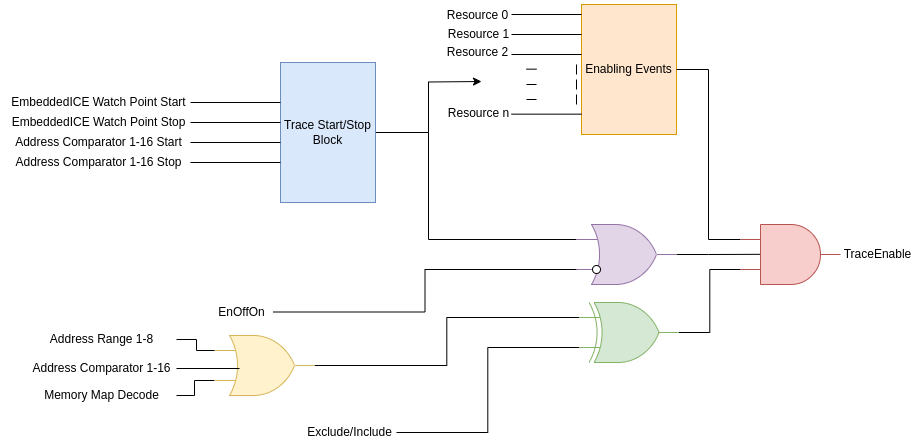
\includegraphics[width=1.00\columnwidth]{etm.drawio.png}
        \caption{TraceEnable Signal Generation}
        \label{fig:TraceEnable}
    \end{figure}
\end{frame}

\begin{frame}
    \frametitle{Consideration for Advanced Processors}
    Parallel execution happens when there are more than one instructions
    executing in one cycle. A little bit of extra trace is possible.
    \begin{itemize}
        \item If the instruction would be traced in the sequential execution,
            then it must be traced in the parallel execution mode.
            Other instruction may be traced in result but nothing should be lost
        \item If the stop address is the first item that is encountered in this
            cycle then the whole cycle is inactive. If it is not then
            the cycle is active.
        \item If the start and stop addresses happen on the same cycle then the
            cycle is active.
    \end{itemize}
\end{frame}

\section{Exploring Timing Capabilities}
\begin{frame}
    \frametitle{Timing in ETM}
    \begin{itemize}
        \item \textit{ETMCR} controls the behavior of the ETM macrocell.
        \item Cycle accuracy is done by setting the bit 12 of the \textit{ETMCR}.
        \item Timestamping also happens in ETM. There are various events that
            cause the ETM module to generate a timestamp packet in the trace
            (T-Sync Packet).
            \begin{itemize}
                \item Enables us to correlate between different trace streams.
                \item Simple analysis of code performance.
                \item Faster search in large trace buffers for code executed
                    in close proximity.
                \item Timestamps are generated in a priodic way.
                    It is controlled by \textit{ETMSYNCFR}.
            \end{itemize}
    \end{itemize}
\end{frame}

\begin{frame}
    \frametitle{Instruction Tracing Representation}
    \begin{itemize}
        \item Instruction Tracing is represented by:
            \begin{itemize}
                \item P-Header packets.
                \item Branch packets (Indirect branch).
                \item Context ID packets (Indicate change in memory map or
                    executing process).
            \end{itemize}
        \item Cycle Accuracy is enabled by \textit{ETMCR}.
            \begin{itemize}
                \item Represented in P-Header packets.
                    \begin{itemize}
                        \item E: Instruction is executed and condition code is
                            passed.
                        \item N: Failed condition test.
                        \item W: Cycle boundary.
                        \item Example: WEWEWNWEE, WWEWWWE.
                    \end{itemize}
                \item Synchronization continues with I-Sync packets.
                \item Cycle count is stored in 32 bit values.
                \item Overflowing in cycle count causes the trace to be
                    inaccurate.
                \item Complex Processors may output different cycles because
                    their different stages proceed independently of others.
            \end{itemize}
    \end{itemize}
\end{frame}

\section{FrankenTrace}
\begin{frame}
    \frametitle{Introduction}
    \begin{itemize}
        \item Tracing: Ability to obtain a detailed record of how software is
            executed by an SoC's processor.
        \item Combined with the binary we can have a full record of the
            subsequently executed instructions.
        \item To examine data transfers an LSU trace is needed. It stores
            addresses, values, and directions of data transfers.
        \item Where we need it:
            \begin{itemize}
                \item Software debugging.
                \item Research reproducability
                \item Post-mortem analysis.
                \item Emulators.
                \item Timinig issues and precise benchmarking.
            \end{itemize}
    \end{itemize}
\end{frame}

\begin{frame}
    \frametitle{Ideas}
    \begin{itemize}
        \item What this paper presents:
            \begin{itemize}
                \item FrankenTrace a tool for non-invasive cycle-level PC and
                    trace and LSU trace of some level of invasiveness.
                \item Only use low speed components that are present in cheap
                    MCUs (DWT, ITM, SWO) and use cheap logic
                    analyzers (FT232RL).
                \item Calls itself accurate cycle-level PC trace using
                    low-speed debugging hardware.
                \item Calls ETM unreliable due to buffer overflows.
                \item Their method is based on repeatability.
                \item Requires each run to be identical.
            \end{itemize}
    \end{itemize}
\end{frame}

\begin{frame}
    \frametitle{Data Watchpoint and Trace: DWT}
    The DWT is an optional debug unit that provides watchpoints, data tracing,
    and system profiling for the processor.
    \begin{itemize}
        \item Can be used as an ETM trigger.
        \item PC sampler event trigger.
            \begin{itemize}
                \item Events can be passed to ITM and make the processor
                    into the debug state.
            \end{itemize}
        \item Data address sampler event trigger.
        \item Has counters for:
            \begin{itemize}
                \item Clock cycles
                \item LSU operations
                \item Sleep cycles
                \item CPI
                \item Interrupt overhead
            \end{itemize}
    \end{itemize}
\end{frame}

\begin{frame}
    \frametitle{DWT Register Map}
    \begin{itemize}
        \item Intended for smaller Cotext-M processors like Cortex-M0
        \item \textit{DWT\_CYCCNT} counts the cycles while the processor is
            not in the debug state.
        \item \textit{DWT\_CPICNT} Additional cycles required to execute
            multi-cycle instructions, and instruction fetch stalls.
        \item \textit{DWT\_EXCCNT} Cycles spent performing exception entry
            and exit procedures.
        \item \textit{DWT\_SLEEPCNT} Cycles spent sleeping
        \item \textit{DWT\_LSUCNT} Cycles spent waiting for loads and stores
            to complete.
        \item \textit{DWT\_FOLDCNT} Cycles saved by instructions which execute in
            zero cycles
        \item Counting instructions using these metrics is approximate
            according to the arm manual.
    \end{itemize}
\end{frame}

\begin{frame}
    \frametitle{Instrumentation Trace Macrocell}
    The ITM is a an optional application-driven trace source that supports
    printf style debugging to trace operating system and application events,
    and generates diagnostic system information.
    \begin{itemize}
        \item Can be used to produce software trace.
        \item Outputing DWT generated packets.
        \item Timestamping with the same source as ETM.
    \end{itemize}
\end{frame}

\begin{frame}
    \frametitle{ETM vs ITM and DWT combo}
    \begin{itemize}
        \item ETM does accurate trace without repetition.
        \item ETM is available on high end SoCs (According to the paper).
        \item ETM needs highspeed, high cost analyzers to mitigate the buffer
            overflow problem (This could be fixed by building a trace
            interface like eg. orbtrace).
        \item Does not need repetition to achieve what it should do.
    \end{itemize}
\end{frame}

\begin{frame}
    \frametitle{Ensuring Repeatablitiy}
    \begin{itemize}
        \item FrankenTrace relies on repeated execution.
        \item Modern SoCs are inherently non-deterministic.
        \item How FrankenTrace solves this:
            \begin{itemize}
                \item Asynchronous clocks are derived from a single clock
                    source using dividers.
                \item Timing that cannot be controlled by microcontroller
                    like sensors are solved by adding resynchronization
                    routine.
                \item Reset the SoC between each repetitiion using
                    \textit{VECTRESET} or \textit{SYSRESETREQ}.
                \item Execute memory and instruction barriers at the start of
                    the execution and flush memory bus buffers.
            \end{itemize}
    \end{itemize}
\end{frame}

\begin{frame}
    \frametitle{What Can We Conclude}
    \begin{itemize}
        \item ETM buffer issues are to be considered (384Mbps for 4 bit TPIU).
        \item Ensuring repeatability is not an easy feat.
        \item Complex tracing environment should be used to advanced the work
            done here (Probably using ETM with HTM). 
        \item Power tracing capabilities was not explored in this presentation.
        \item how should we define the invasiveness of tracing environment.
        \item Pricing for a TPIU trace unit:
            \begin{itemize}
                \item 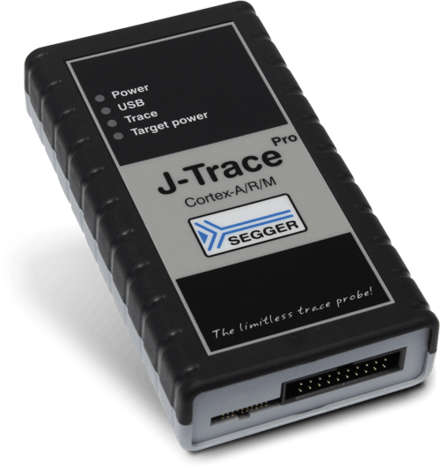
\includegraphics[width=1.3cm,valign=c]{jtraceARM.png} J-Trace Cortex-A/R/M, 1980 EUR.
                \item 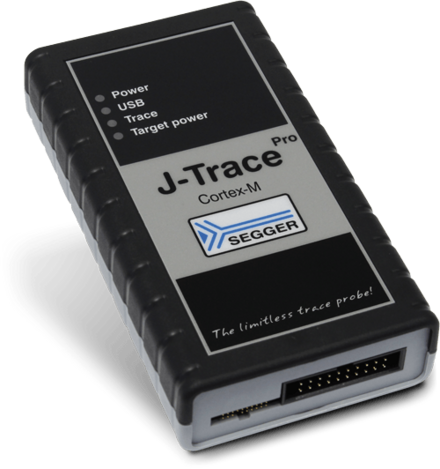
\includegraphics[width=1.3cm,valign=c]{jtraceM.png} J-Trace Cortex-M, 1490 EUR.
                \item 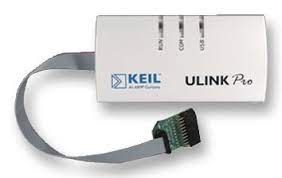
\includegraphics[width=1.3cm,valign=c]{ulink.jpeg} Keil ULINKpro (not ULINKpro D), 987 EUR.
            \end{itemize}
    \end{itemize}
\end{frame}

\begin{frame}
    \frametitle{OrbTrace}
    \begin{figure}
        \centering
        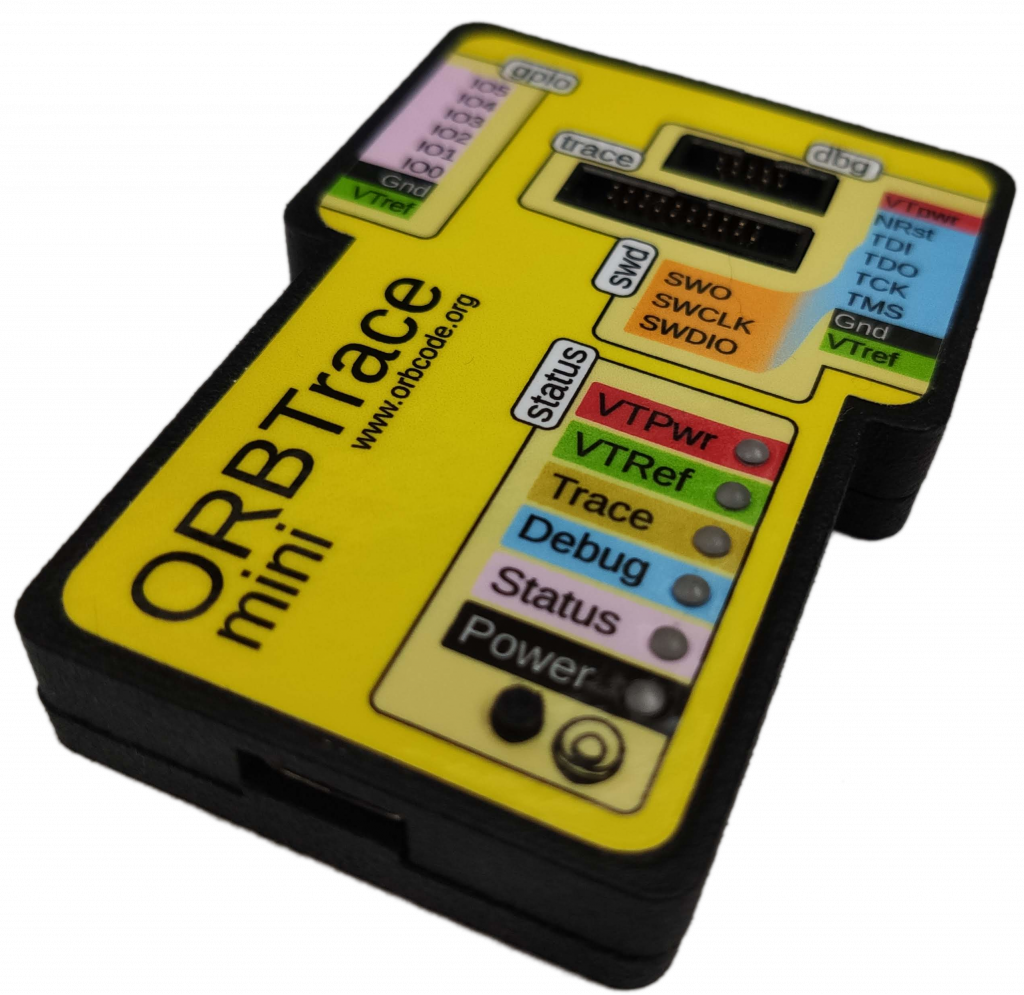
\includegraphics[width=0.5\columnwidth]{orbtrace.png}
        \caption{OrbTrace Debug and Parallel Trace interface}
        \label{fig:orbtrace}
    \end{figure}
\end{frame}

\begin{frame}
  \centering \Large
  \emph{Thank You For Your Attention}
\end{frame}

\end{document}
